
\documentclass[letterpaper]{article}
\usepackage{underscore}
\usepackage[left=2.5cm, right=2.5cm, top=2cm]{geometry}
\usepackage[utf8]{inputenc}
\usepackage{graphicx}
\usepackage{graphics}
\usepackage[spanish]{babel}
\usepackage{lipsum}
\usepackage{float}
\usepackage{subfigure}
\usepackage{csquotes}
\usepackage{color}
\usepackage{colortbl}
\usepackage{xcolor}
\usepackage{multirow}

\title{Diagrama eléctrico de la interfaz de potencia}
\author{Alcantar Díaz Joel Alejandro\\ Carrasco Quiñones Karla Daniela\\ Ledesma Hernández Miguel Ángel\\  Reyna Gurrola Marcela\\ }
\date{10/Noviembre/2019}

\begin{document}

\maketitle
\vspace{2cm}
\begin{large}
    \begin{center}
        
\includegraphics[scale=0.5]{IMG/UPZMGlog.png}
    \end{center}
\end{large}
\vspace{2cm}
\begin{center}
4-A Mecatrónica\\
Sistemas Electrónicos de Interfaz   
\end{center}

\newpage

\section{Objetivo}
\begin{large}
    Armar una fuente conmutada funcional con un buck a la salida.
\end{large}

\section{Materiales}
\begin{table}[hbtp]
    \centering
    \begin{tabular}{|l|l|}
    \hline
       {\color[HTML]{3166FF}\textbf{Equipo}}  &   {\color[HTML]{CB0000}\textbf{Componentes}}\\ \hline
        Multímetro  & Mosfet IRF640N\\ \hline
        Protoboards  & Resistencias varias \\ \hline
        Computadora & Cables \\ \hline
        Fuente      & LM555   \\ \hline
                    & Transformador    \\ \hline
                    & Inductor 2.2mH   \\ \hline
                    & Capacitores electrolíticos\\\hline
                    & Diodos\\\hline
                    & SCR S4015J\\\hline
                    & Capacitores cerámicos\\\hline
                    & Potenciómetro de 100K \\\hline
    \end{tabular}
    \caption{Material utilizado}
    \label{tab:materiales}
\end{table}


\section{Procedimiento}
\begin{enumerate}
    \item En primera instancia toma el transformador y conéctalo directamente al enchufe, para medir sus salidas y decidir cuanto voltaje de entrada se va a rectificar.
    \begin{figure}[htbp]
        \centering
        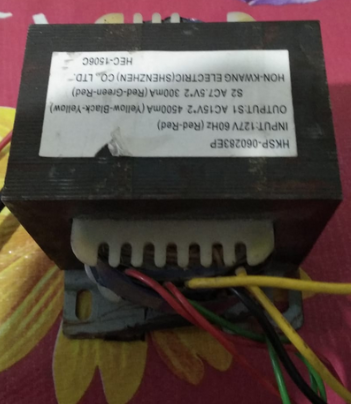
\includegraphics[scale=.5]{IMG/trans.PNG}
        \caption{Transformador}
        \label{fig:trans}
    \end{figure}
        
    
    \item Crea un circuito usando los LM555 para regular el disparo de los gatillos del SCR cuando estén en proceso de rectificación en compañía de dos diodos.
    \begin{figure}[htbp]
        \centering
        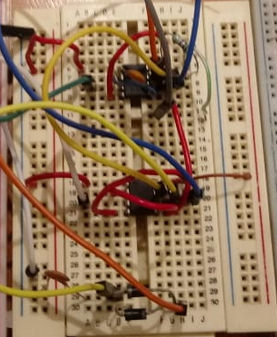
\includegraphics{IMG/555supergenial.PNG}
        \caption{Circuito final 555 con rectificador de diodos}
        \label{fig:lm5555555}
    \end{figure}
    
    \item De esta manera conecta el transformador al circuito de rectificación formado por los dos SCR's y los diodos, el cual será un puente rectificador semicontrolado.\\
    \begin{figure}[htbp]
        \centering
        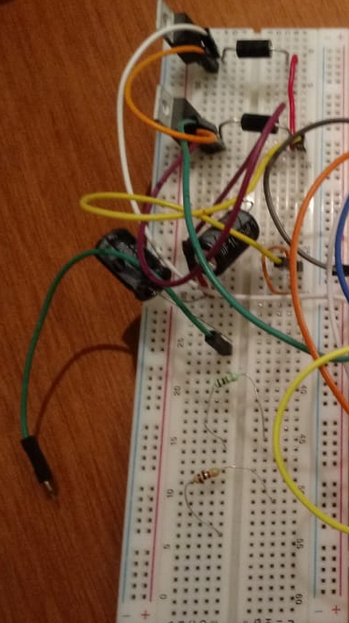
\includegraphics[scale=.7]{IMG/scrsgeniales.PNG}
        \caption{SCR's con diodos}
        \label{fig:my_label}
    \end{figure}
    \item Conectar en la toma de corriente para medir voltajes en las salidas y comprobar si funciona correctamente el rectificador y los circuitos de activación con lo 555, cabe mencionar que estos se alimentarán con 5V. \\
    (Para probar si en circuito oscilador funciona se conecta un motor, si el circuito funciona la velocidad del motor disminuirá o aumentara dependiendo de la velocidad de oscilación, la cual se controla con ayuda de un potenciómetro).
   \item Por último, conecta la salida del rectificador ya filtrada, con ayuda de un par de capacitores, para hacer el ajuste fino del voltaje, es decir, el boost, cuk o en este caso el buk.
   
\end{enumerate}

\section{Resultados}
\begin{large}
    Por desgracia la fuente no funcionó del todo bien, en la etapa de rectificación secundaria o ajuste fino el circuito fallo. Anteriormente el circuito había sido probado de manera independiente y funcionó pero al conectarlo de nuevo falló y no se pudo "echar a andar" de nuevo ni solo.\\
    Las otras dos partes  del circuito funcionaban a la perfección, los 555 daban el pulso necesario y el rectificador cumplía su labor de bajar el voltaje y convertirlo a directo.
\end{large}


\begin{figure}[htbp]
    \centering
    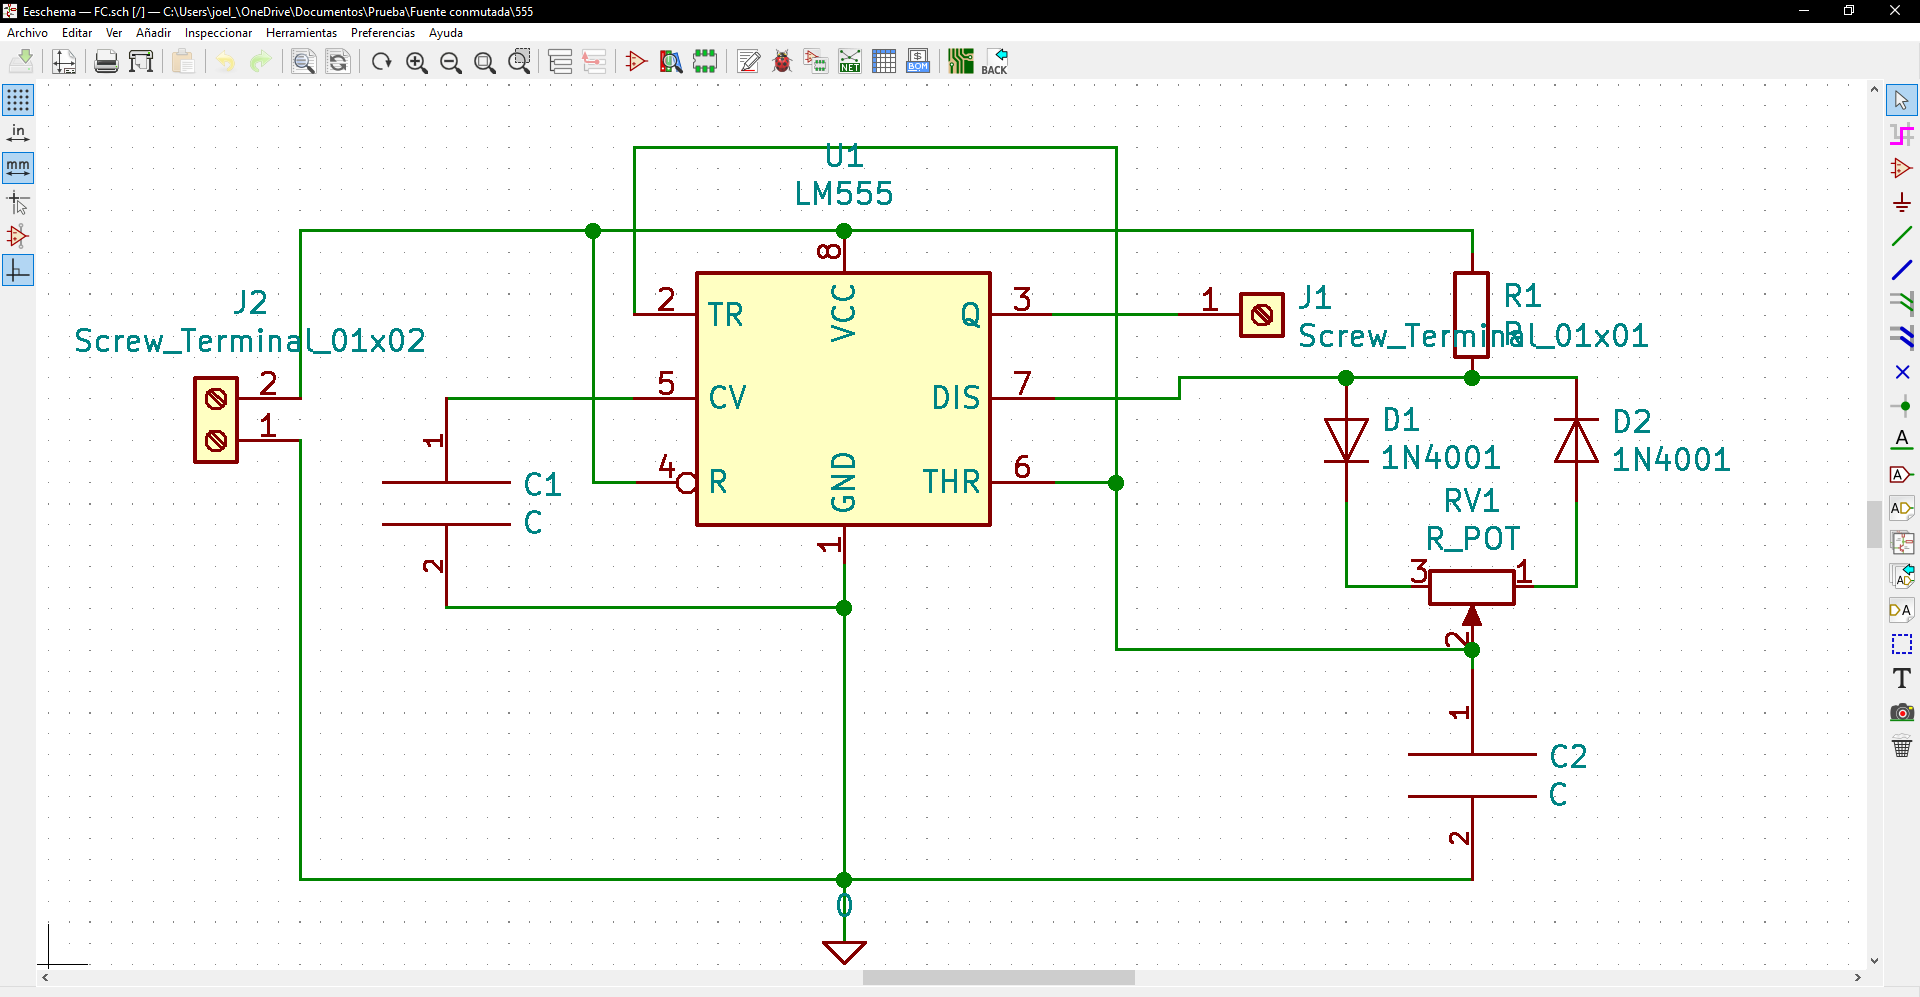
\includegraphics[scale=0.2]{IMG/555.png}
    \caption{Circuito PWM.}
    \label{fig:PWM}
\end{figure}

\begin{figure}[htbp]
    \centering
    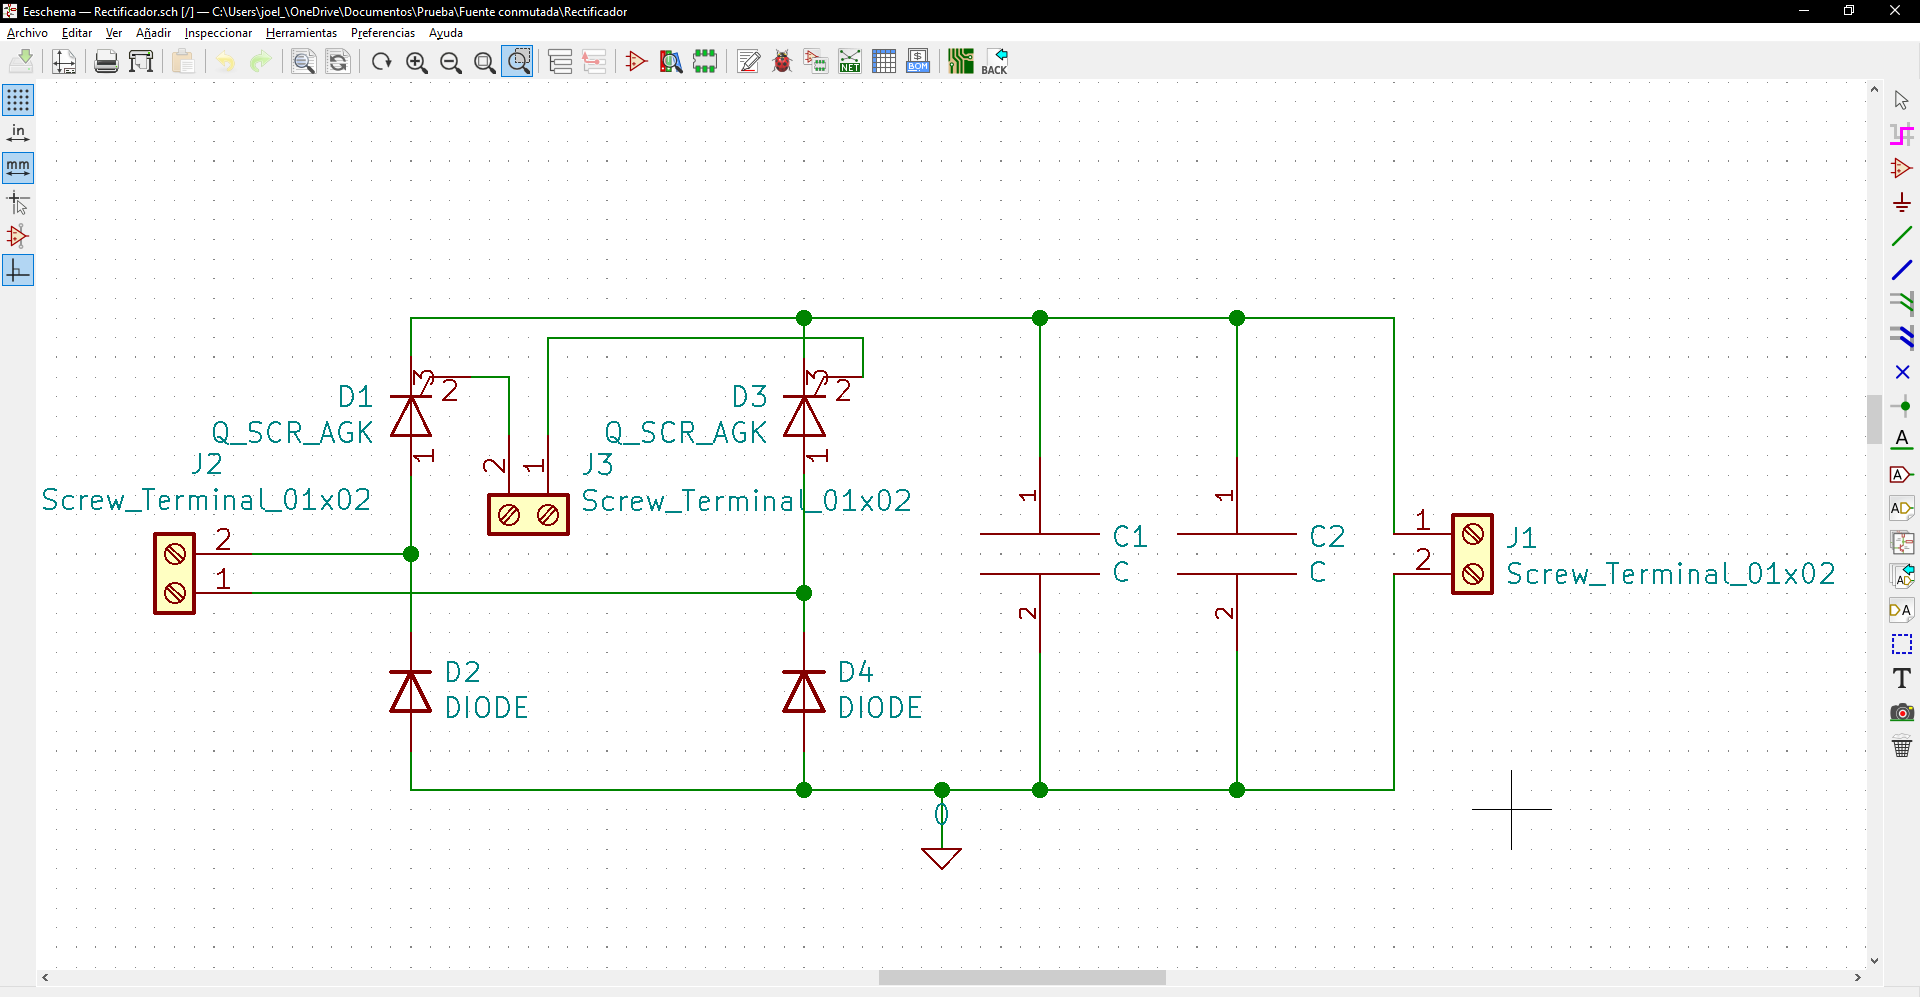
\includegraphics[scale=0.2]{IMG/rectificador.png}
    \caption{Circuito rectificador semi-controlado.}
    \label{fig:SCR}
\end{figure}

\newpage

\begin{figure}[htbp]
    \centering
    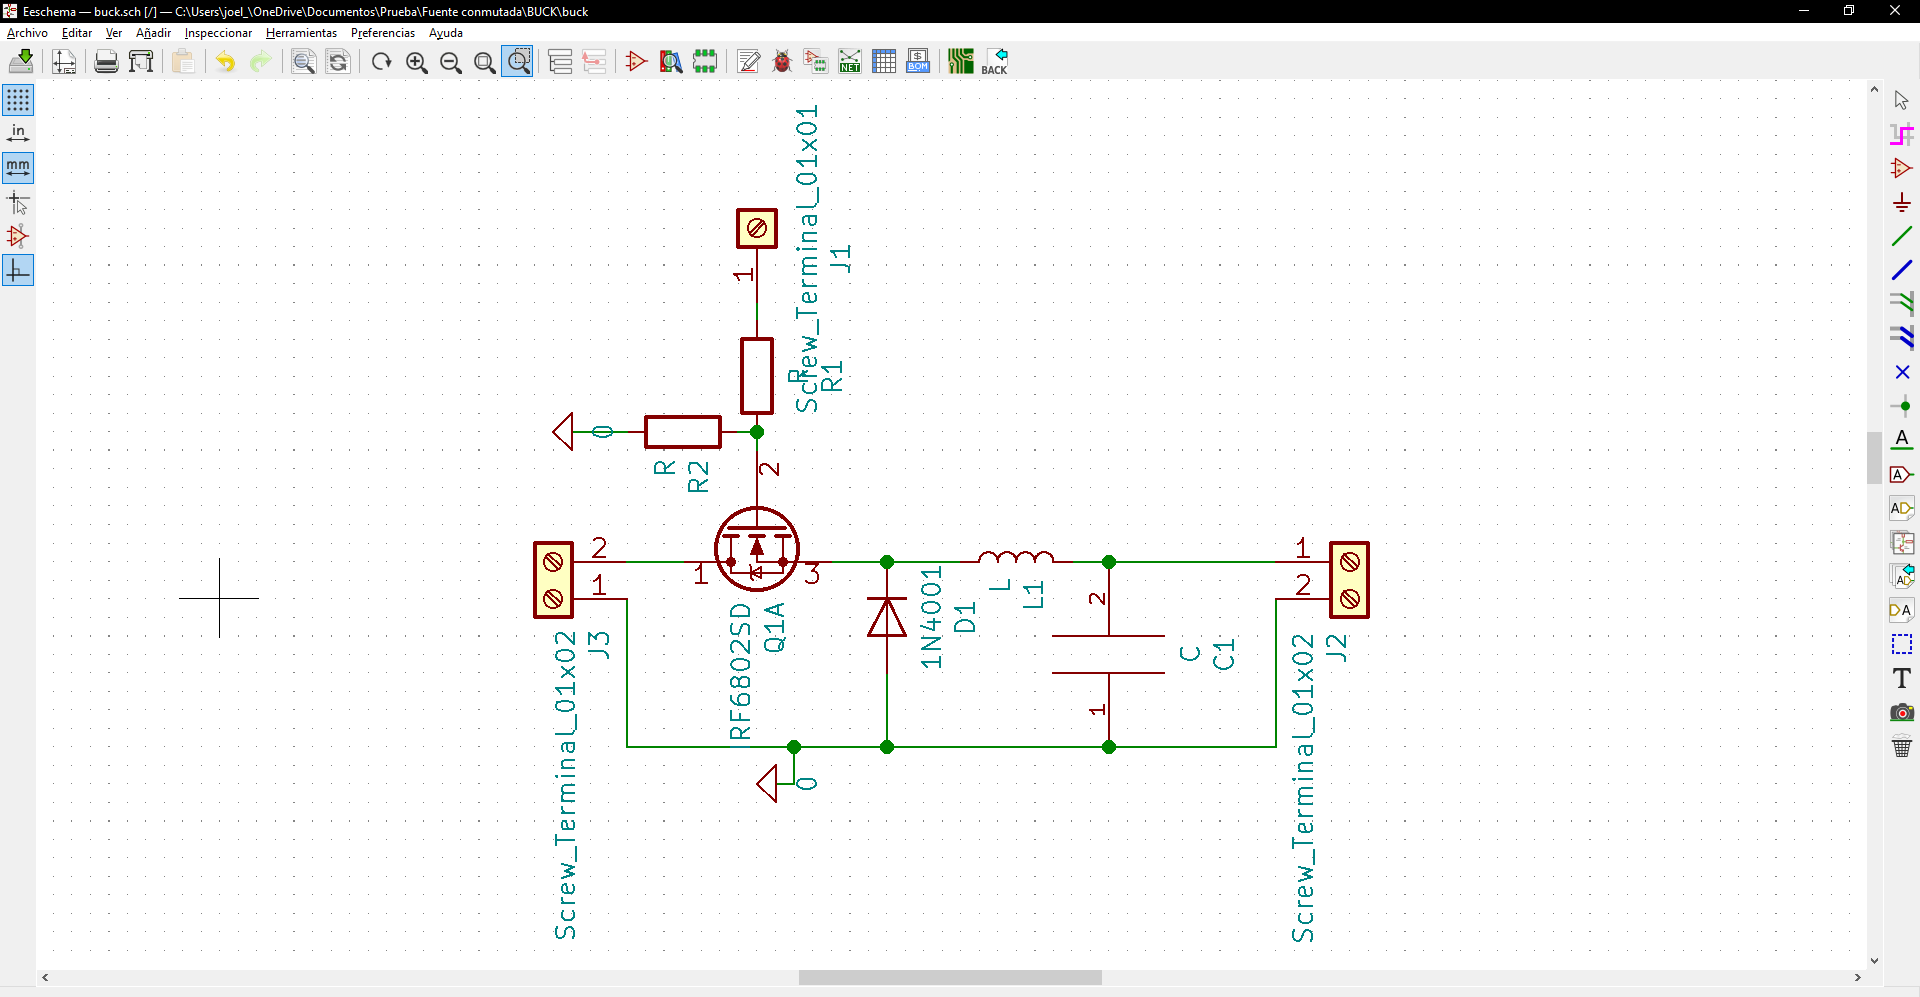
\includegraphics[scale=0.2]{IMG/buk.png}
    \caption{Circuito reductor de voltaje.}
    \label{fig:BUKY}
\end{figure}

\begin{figure}[htbp]
    \centering
    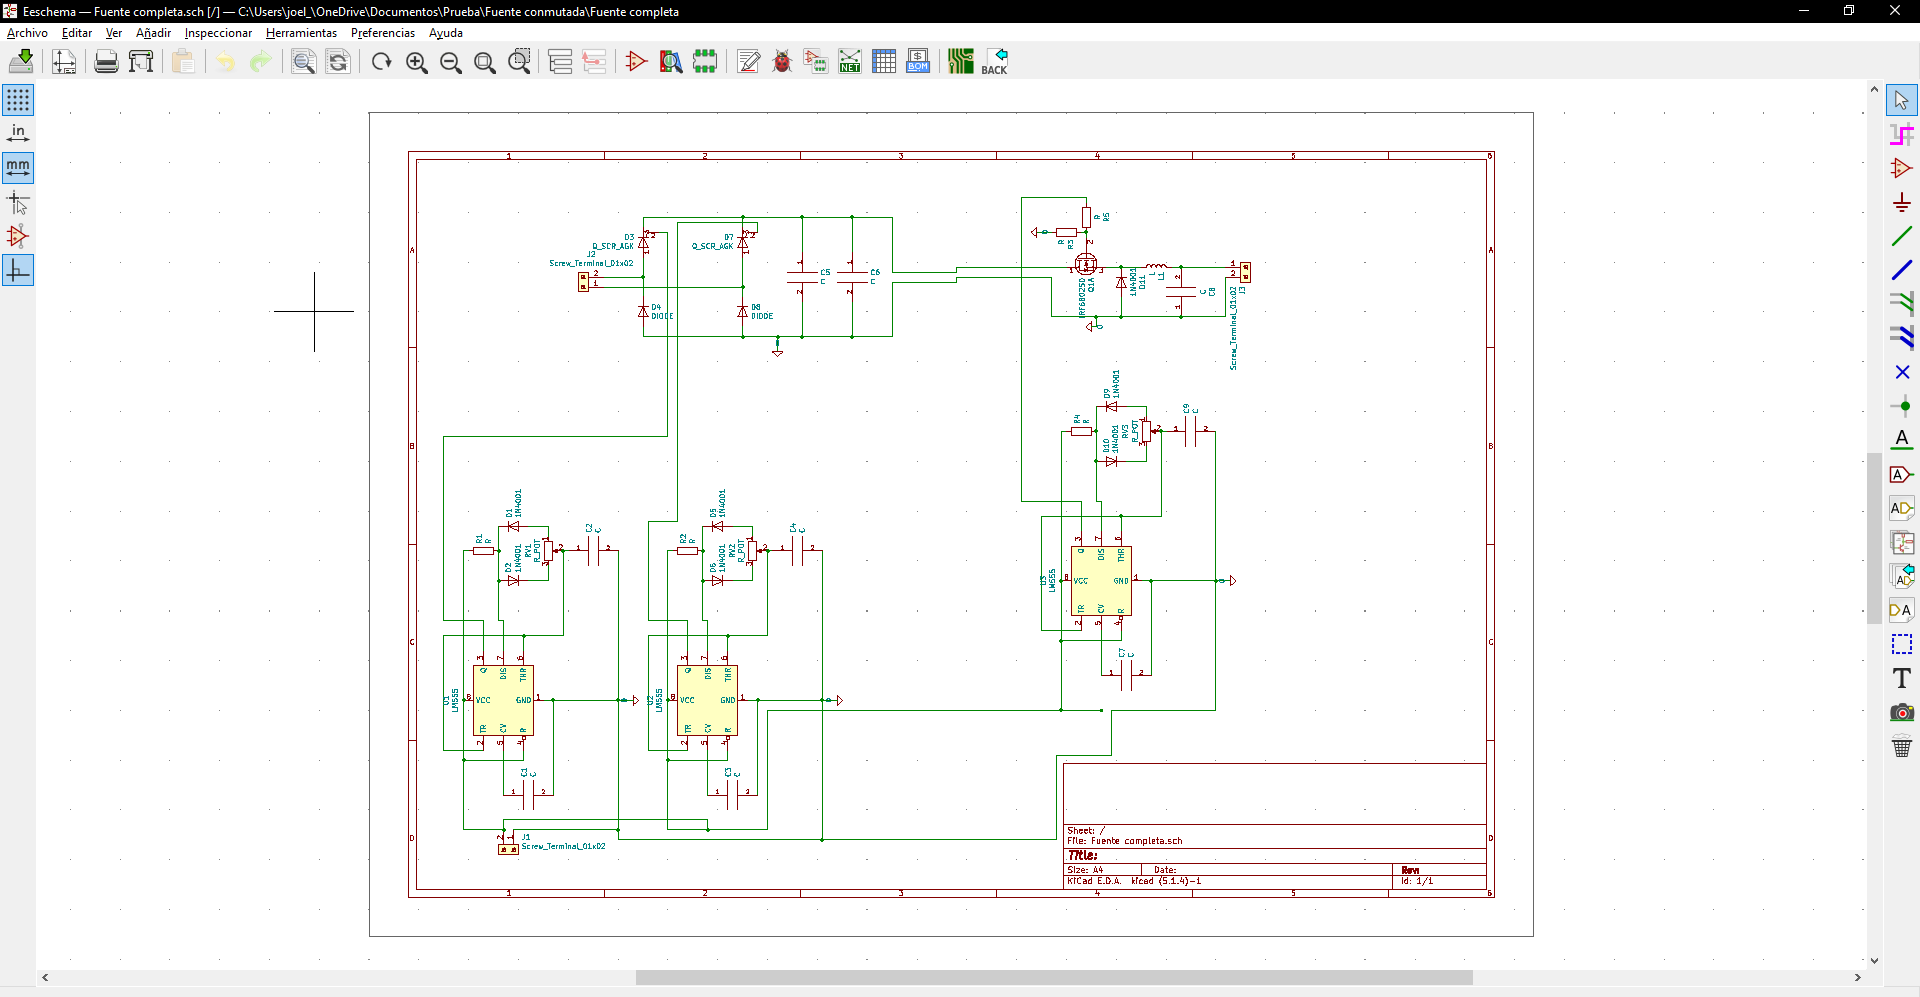
\includegraphics[scale=0.2]{IMG/fuentecompleta.png}
    \caption{Circuito final.}
    \label{fig:FuenteBB}
\end{figure}

\newpage

\subsection{Evidencias:}
\begin{figure}[htbp]
    \centering
    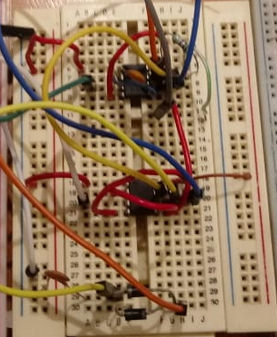
\includegraphics[scale=1]{IMG/555supergenial.PNG}
    \caption{Circuito con LM555 armado.}
    \label{fig:555}
\end{figure}

\begin{figure}[htbp]
    \centering
    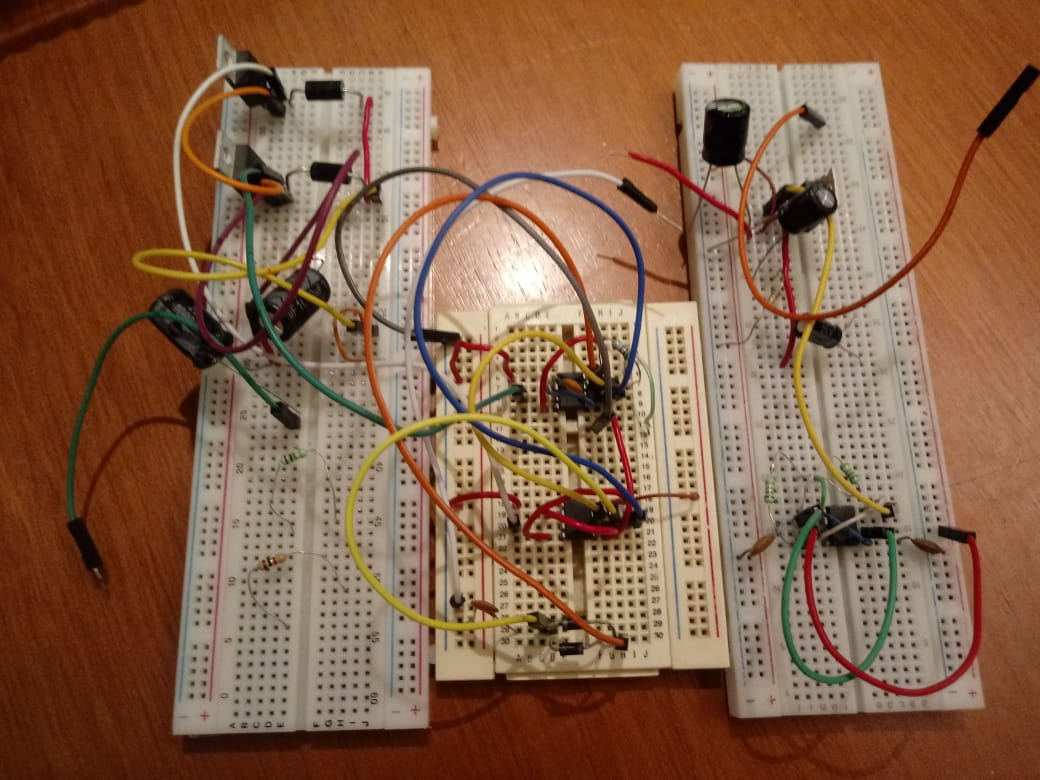
\includegraphics[scale=0.2]{IMG/FinalFisico.jpeg}
    \caption{Fuente terminada}
    \label{fig:Allaenlafuente}
\end{figure}

\newpage
\section{Conclusión}
\textbf{Alcantar Díaz Joel Alejandro:\\}
\begin{large}
    Para el correcto funcionamiento del oscilador con los SCR es necesario conectar todas las tierras al mismo lugar, de igual manera con el MOSFET.\\
    Para el MOSFET se necesita poner una resistencia de "desagüe" por decirlo de una manera que condusca a tierra ya que queda activado si no se descarga. Esta resistencia tiene que ser mas grande que la que se coloque de base a pulso.\\
    Las bobinas funcionan como Capacitores pero de corriente\\
    La eficiencia de una fuente conmutada es mayor ya que no desperdicia tanta energía en calor como lo hace un circuito resistivo.\\
    El funcionamiento de una fuente conmutada es mas sencillo de lo que esperaba.\\\\
\end{large}



\textbf{Carrasco Quiñones Karla Daniela:\\}
Como nos pudimos dar cuenta en esta práctica es que la fuente conmutada que realizámos en esta ocación es mucho mas facíl que cualquier otra; apredimos el uso correcto y adecuado de las SCR.\\
Descubrimos que esto hace casi el mismo funcionamiento a la de un capacitor, este guerda energía y al mometo de llegar a su capacidad de energía este se vuelve a descargar y así consecutivamente.\\\\
\textbf{Ledesma Hernández Miguel Ángel:\\}
\begin{large}
    Se queda como conocimiento el uso de la conjunción de múltiples tipos de circuito para crear distintos tipos de ondas que pueden ayudar a la creación de sistemas que necesiten de este tipo de ondas.\\
A su vez se aprendió sobre el uso de los transformadores y aplicaciones de inductores en el sistema, como pudimos ver con el inductor de 2.2mH que almacenaba cierto voltaje para darle por así decirlo un "smooth" a la par de los capacitores.\\
Y por ultimo como un conocimiento de práctica el separar los elementos complejos de un circuito complejo para identificar el error en este sistema para posteriormente arreglarlo de manera individual y no perder primeramente tiempo en buscar en todo el circuito.\\\\
\end{large}

\textbf{Reyna Gurrola Marcela:\\}
\begin{large}
La razón por la que se hizo esta fuente conmutada, es que son mucho más eficientes y fáciles de controlar. Ya que con ayuda de los SCRs, en conjunto con los diodos, se puede rectificar una señal mejor evitando pérdidas.\\ Y a pesar de que no funcionó en conjunto con el circuito de ajuste fino se pudo comprender cómo funciona y las partes que conforman a este tipo de fuentes.\\\\
\end{large}




\end{document}
